\documentclass{ecnreport}

\stud{OD Robotique 2023-2024}
\topic{ROS 2 exam}

\begin{document}

\inserttitle{ROS 2 exam}

\insertsubtitle{2h, documents / internet allowed (closed chats please)}


\section{Description}

In this exam you will have to write a C++ node and run it several times through a launch file.\\

The files are split into two packages that you should compile first:

\begin{itemize}
 \item \okt{ecn_usv}: simulates an unmanned surface vehicle. You do not have to modify anything in this package
 \item \okt{ecn_2023}: simulates a world and some drones, this is where you do the work.
\end{itemize}

\begin{figure}[h]\centering
 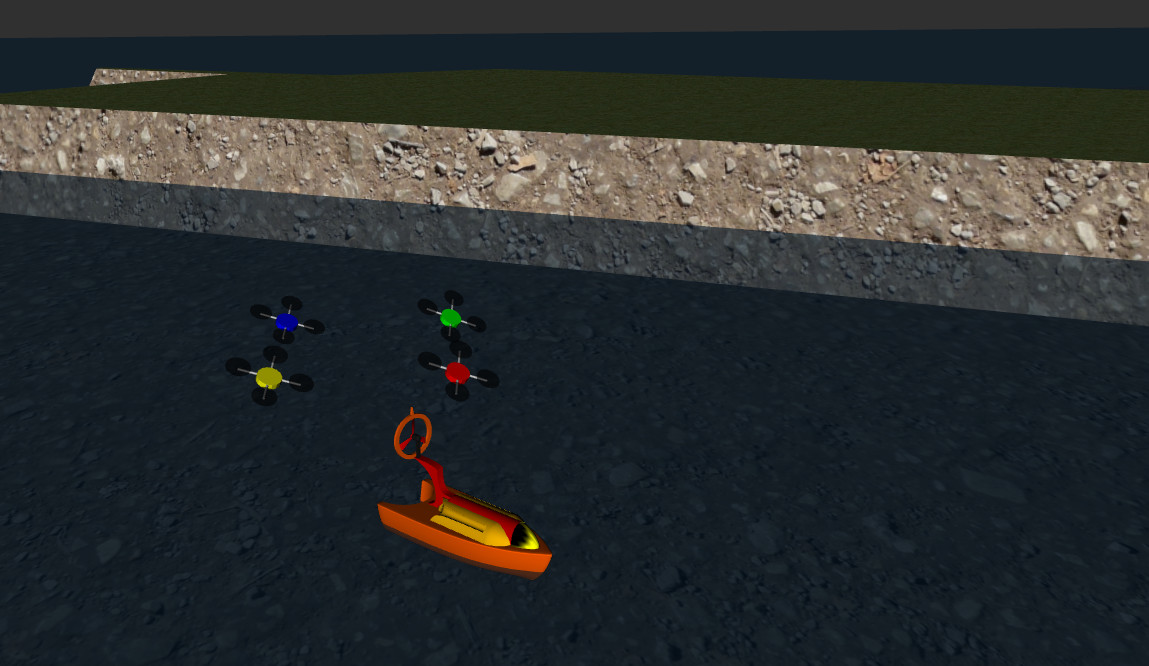
\includegraphics[width=.5\linewidth]{simulation}
\end{figure}

The overall simulation can be run with two commands (to be run in two terminals):
\begin{bashcodelarge}
 ros2 launch ecn_2023 world_launch.py
 ros2 launch ecn_usv usv_launch.py
\end{bashcodelarge}once run there should be no reason to stop it. The drones will go back to their home position if no control is received.


\subsection*{Objectives}

The goal of the exam is to have 4 drones track a suspicious USV moving around an island. To do so, each drone should have a desired position (defined with regards to the USV) and a controller to track this setpoint. The steps are thus:

\begin{itemize}
 \item Write the controller node
 \item Write a launch file that:
 \begin{itemize}
  \item Runs the controller for all drones
  \item Runs static transform broadcaster to define where the drones should be with regards to the USV
 \end{itemize}
\end{itemize}

The nodes should be run in the namespaces \okt{uav1} $\hdots$ \okt{uav4}.

\section{Static transform broadcaster}

The target position of a given UAV is defined with regards to the USV base frame. Such a transformation should be published on \okt{/tf} through a Static transform broadcaster:
\begin{bashcodelarge}
 ros2 run tf2_ros static_transform_publisher
\end{bashcodelarge}
This node takes the following arguments, assuming we set the desired pose for UAV 1:
\begin{itemize}
 \item \okt{--frame-id}: name of the parent frame (\okt{usv/base_link})
 \item \okt{--child-frame-id}: name of the child frame (\okt{uav1/target})
 \item \okt{--x}: X-offset of the pose
 \item \okt{--y}: Y-offset of the pose
 \item \okt{--z}: Z-offset of the pose (15)
\end{itemize}

The X and Y offsets should be set depending on the UAV number:
 \begin{table}[h]\centering
  \begin{tabular}{|c|c|c|}\hline
   Drone & X-offset & Y-offset \\\hline
   1 & 10 & 0 \\\hline
   2& 0 &10 \\\hline
   3 & -10 & 0 \\\hline
   4 & 0 & -10 \\\hline
  \end{tabular}
 \end{table}

 You can run first this static transform publisher in a console for drone 1, to help coding the control node.

\section{Control node}

The control node is written in \okt{uav.cpp}. Parts of the node class are already here.
As usual, it is a good idea to code the control explicitely from a given UAV before making the code generic and use it from a launch file.

\subsection{Inputs / outputs}

The node should:
\begin{itemize}
 \item Declare a parameter to know which UAV is considered (1 to 4)
 \item Declare a publisher to send the controls (use \okt{ros2 topic} to identify it)
 \item Use a service client to retrieve the current error to its target position
 \item Run a controller at a rate of 50 ms
\end{itemize}

Some gains are already declared.

\subsection{Service client}

A service called \okt{/target} is advertized by the \okt{/target_computer} node. The service is of type \okt{ecn_2023/srv/Target}:
\begin{bashcode}
string uav
---
float64 x
float64 y
float64 z
float64 theta
\end{bashcode}
The request should contain the name of the UAV (\okt{uav1} $\hdots$ \okt{uav4}). The response will be the current error $(x,y,z,\theta)$ from the UAV to its target pose.

Calling this service in a synchronous way can be done through the \okt{client} member variable:
\begin{itemize}
 \item Needs to be initialized in the constructor, to be given the name of the service
 \item Can be called with various approaches (see \okt{client_spinner.h}):
 \begin{cppcode}
  // returns an actual ResponseT if the call succeded
  std::optional<ResponseT> call(const RequestT &req)

  // returns True is the call succeded, in this case res is the response
  bool call(const RequestT &req, ResponseT &res)
 \end{cppcode}
\end{itemize}

\subsection{Control}

\newcommand{\var}[1]{\texttt{\upshape #1}}

The control is a basic proportional-integral that takes the error from the service call.
This function should be run at 50 ms.

 \begin{algorithm}[!h]
 \DontPrintSemicolon
 \SetKwFunction{Fill}{{\bf Function} updateControl}\;
 \Fill{}
 {
 \\
 Call service to get current error, named \var{error} here\;
 \If{Service call failed}{\Return;}
 \tcp{Integral error for x and y}
 $ei_x \gets ei_x + \var{error.x}$ \;
 $ei_y \gets ei_y + \var{error.y}$ \;
 \tcp{Compute desired velocity}
 $v_x \gets K_p*\var{error.x} + K_i*ei_x$ \;
 $v_y \gets K_p*\var{error.y} + K_i*ei_y$ \;
 $v_z \gets K_p*\var{error.z}$ \;
 $\omega_z \gets K_w*\var{error.theta}$ \;
 Publish velocity command $(v_x,v_y,v_z,\omega_z)$\;
}
% \SetAlgoLined
\caption{UAV Control}
\label{backtracking}
\end{algorithm}

\newpage
\section{The launch file}

Once your node runs for a given drone, write a launch files that runs the node and the static transform publisher for the 4 drones.

\paragraph{Tip} You can use a loop for the drone number and get the corresponding namespace:
\begin{pythoncode}
    for i in (1,2,3,4):
        ns = f'uav{i}'
        # do stuff in this namespace
        # use i to run static_transform_publisher with correct arguments
\end{pythoncode}

\section{Bonus: super launch launch file}

Once everything works, you may also write a super-launch file that runs everything in one command:
\begin{itemize}
 \item include \okt{world_launch.py}
 \item include \okt{usv_launch.py}
 \item include your own launch file for the UAV's
\end{itemize}

In order to reduce oscillations for the USV, the \okt{usv_launch.py} file can be passed better gains when included:
\begin{itemize}
 \item ~\okt{Kv} argument can be set to 4.
 \item ~\okt{Kw} argument can be set to 1.2
\end{itemize}


\end{document}
